% !TeX document-id = {6b928c0d-85af-41d1-a21b-e6c7a23a6e8d}
% !TeX TXS-program:compile = txs:///pdflatex/[--shell-escape]

%include guard:
\ifdefined\GlobalAlreadyIncluded
  \expandafter\endinput
\fi

\gdef\GlobalAlreadyIncluded{}
%

\documentclass[accentcolor=3c,landscape,ngerman,presentation,t,usenames,dvipsnames,svgnames,table, aspectratio=169]{tudabeamer}

% Template-Modifikationen
\addtobeamertemplate{frametitle}{}{\vspace{-1em}} % mehr Platz vor dem Inhalt

% andere global gemeinsame definitionen
%Includes
\usepackage[ngerman]{babel} %Deutsche Silbentrennung
\usepackage[utf8]{inputenc} %Deutsche Umlaute
\usepackage{float}
\usepackage{graphicx}
\usepackage{minted}

\DeclareGraphicsExtensions{.pdf,.png,.jpg}

\makeatletter
\author{Vorkursteam der Fachschaft Informatik}
\let\Author\@author

% dark Mode
\ExplSyntaxOn
\RequirePackage{pagecolor,xcolor, graphicx} % Used for dark Mode
\bool_gset_false:N \g_dark_mode_bool % Disable by default
\newcommand{\enableDarkMode}{ %Command to enable Dark Mode (only works before \begin{document})
	\definecolor{anthrazitgrau}{HTML}{293133}
	\pagecolor{anthrazitgrau}
	\color{white}

	\cs_if_exist:NT \setbeamercolor {
		\setbeamercolor*{smallrule}{bg=.}
		\setbeamercolor*{normal~text}{bg=,fg=.}
		\setbeamercolor*{background canvas}{parent=normal~text}
		\setbeamercolor*{section~in~toc}{parent=normal~text}
		\setbeamercolor*{subsection~in~toc}{parent=normal~text,fg=\thepagecolor}
		\setbeamercolor*{footline}{parent=normal~text}
		\setbeamercolor{block~title~alerted}{fg=white,bg=white!20!\thepagecolor}
		\setbeamercolor*{block~body}{bg=white!10!\thepagecolor}
		\setbeamercolor*{block~body~alerted}{bg=\thepagecolor}
	}
	\cs_if_exist:NT \setbeamertemplate {
		\setbeamertemplate{subsection~in~toc~shaded}[default][50]
	}
	\bool_gset_true:N \g_dark_mode_bool
	% Prefer inverted Logo with dark Mode
	% \IfFileExists{tuda_logo_inverted.pdf}{\tl_gset:Nn \g_ptxcd_logofile_tl {tuda_logo_inverted.pdf}}{}
	% \hbox_gset:Nn \g__ptxcd_logo_box {% Update Logo Box
	% 	\makebox[2.2\c_ptxcd_logoheight_dim][l]{\includegraphics[height=\c_ptxcd_logoheight_dim]{\g_ptxcd_logofile_tl}}%
	% }
}

% dark Mode Makros
\prg_new_conditional:Nnn \__ptxcd_if_dark_mode: {T,F,TF} { % Conditional to check if dark Mode is active
	\bool_if:NTF \g_dark_mode_bool
	{\prg_return_true:}
	{\prg_return_false:}
}

\cs_set_eq:NN\IfDarkModeT \__ptxcd_if_dark_mode:T % Easy dark Mode check for use in document
\cs_set_eq:NN\IfDarkModeF \__ptxcd_if_dark_mode:F
\cs_set_eq:NN\IfDarkModeTF \__ptxcd_if_dark_mode:TF

\newcommand{\includeinvertablegraphics}[2][]{% Grafik wird beim Dark Mode automatisch Invertiert (rgb)
	\IfDarkModeTF{\includegraphics[decodearray={1.0~0.0~1.0~0.0~1.0~0.0},#1]{#2}}{\includegraphics[#1]{#2}}
}
\newcommand{\includeinvertablegrayscalegraphics}[2][]{% Grafik wird beim Dark Mode automatisch Invertiert (grayscale)
	\IfDarkModeTF{\includegraphics[decodearray={1.0 0.0},#1]{#2}}{\includegraphics[#1]{#2}}
}

% DARK_MODE environment check (enable if DARK_MODE=1)
\sys_get_shell:nnN { kpsewhich ~ --var-value ~ DARK_MODE } { } \l_dark_mode_env_var_tl
\tl_trim_spaces:N \l_dark_mode_env_var_tl
\tl_if_eq:NnT \l_dark_mode_env_var_tl {1} {\enableDarkMode{}}
\ExplSyntaxOff

% macros
\renewcommand{\arraystretch}{1.2} % Höhe einer Tabellenspalte minimal erhöhen
\newcommand{\N}{{\mathbb N}}
\newcommand{\code}{\inputminted[]{python}}
\newmintedfile[pythonfile]{python}{
	fontsize=\small,
	style=\IfDarkModeTF{fruity}{friendly},
	linenos=true,
	numberblanklines=true,
	tabsize=4,
	obeytabs=false,
	breaklines=true,
	autogobble=true,
	encoding="utf8",
	showspaces=false,
	xleftmargin=20pt,
	frame=single,
	framesep=5pt,
}
\newmintinline{python}{
	style=\IfDarkModeTF{fruity}{friendly},
	encoding="utf8"
}

\definecolor{codegray}{HTML}{eaf1ff}
\newminted[bashcode]{awk}{
	escapeinside=||,
	fontsize=\small,
	style=\IfDarkModeTF{fruity}{friendly},
	linenos=true,
	numberblanklines=true,
	tabsize=4,
	obeytabs=false,
	breaklines=true,
	autogobble=true,
	encoding="utf8",
	showspaces=false,
	xleftmargin=20pt,
	frame=single,
	framesep=5pt
}

\let\origpythonfile\pythonfile
\renewcommand{\pythonfile}[1]{\pythonfileh{#1}{}}
\newcommand{\pythonfileh}[2]{\origpythonfile[#2]{#1}}

\newcommand*{\ditto}{\texttt{\char`\"}}

%Includes
\usepackage{epstopdf}
\usepackage{wrapfig}
\usepackage{tipa}
\usepackage{tikz}
\usetikzlibrary{calc,shapes,arrows}
%tip: use http://l04.scarfboy.com/coding/phonetic-translation?from=ipa&fromtext=%CB%88pa%C9%AA%CE%B8n%CC%A9&to=tipa
%for converting ipa

\graphicspath{ {./media/} }

\def\shortyear#1{\expandafter\shortyearhelper#1}
\def\shortyearhelper#1#2#3#4{#3#4}

\newcount\NextYear
\NextYear = \year
\advance\NextYear by 1

\newcommand\NextYearShort{\shortyear{\the\NextYear}}

% notes
\usepackage{pgfpages}
\setbeamertemplate{note page}[plain]
%\setbeameroption{show notes on second screen}

% macro for change speaker sign
\newcommand{\changespeaker}{
	\begin{tikzpicture}[line width=.6mm, shorten >= 3pt, shorten <= 3pt]

		\coordinate (c1);
		\coordinate[right of=c1] (c2);

		\draw[rectangle, draw=red!80, fill=red!80, align=center, rounded corners] ($(c1.north west)+(0,-0.3)$) rectangle ($(c2.south east)+(0, 0.3)$) {};
		\draw[->,white] (c1)[bend left] to node[auto] {} (c2);
		\draw[->,white] (c2)[bend left] to node[auto] {} (c1);
	\end{tikzpicture}
}

%Listing-Style pyhon
\title[Programmiervorkurs]{Programmiervorkurs Wintersemester \the\year/\NextYearShort}
\subtitle{{\small der Fachschaft Informatik}}
\logo*{
\includegraphics{../globalMedia/bildmarke_ohne_rand}}
\institute{Fachschaft Informatik}
\date{Wintersemester \the\year/\NextYearShort}


% macros
\newcommand{\livecoding}{
		\ifdefined\StreamSlides
			\begin{frame}
				\frametitle{\insertsectionhead \\  {\small \insertsubsectionhead}}\centering \huge 	\vskip 2cm\textbf{\textcolor{red}{Live-Coding}}
			\end{frame}
		\fi
	}

%\newcommand{\slidehead}{\frametitle{\insertsectionhead \\ {\small \insertsubsectionhead}}\vspace{3mm}}
\newcommand{\slidehead}{\frametitle{\insertsectionhead} \framesubtitle{\insertsubsectionhead}\vspace{3mm}}
\newcommand{\tocslide}{\begin{frame}[t]\frametitle{Inhaltsverzeichnis}\vspace{3mm}{\small\tableofcontents[subsectionstyle=shaded]}\end{frame}}

\newcommand{\nextvid}[2]{
	\ifdefined\StreamSlides
	\else
		\section{Nächstes Video}
		\begin{frame}[t]
			\slidehead
			\begin{block}{Nächstes Video}
				\vspace{0.5cm}
				#1
				\vspace{0.5cm}
			\end{block}
			\ifx\hfuzz#2\hfuzz
				\vspace{2.5cm}
			\else
				{\begin{block}{Bonus Video}
					\vspace{0.5cm}
					#2
					\vspace{0.5cm}
				\end{block}}
			\fi
			Danke fürs Zuschauen!\\
			Links zu den Folien und Quellen sind in der Videobeschreibung.
		\end{frame}
	\fi
}


\usepackage{verbatim}
\usetikzlibrary{decorations.pathreplacing}
\usetikzlibrary{shapes.misc}


% colors
\definecolor{lightpetrol}{RGB}{0,223,194}

% dark Mode
\ExplSyntaxOn
\RequirePackage{pagecolor,xcolor, graphicx} % Used for dark Mode
\bool_gset_false:N \g_dark_mode_bool % Disable by default
\newcommand{\enableDarkMode}{ %Command to enable Dark Mode (only works before \begin{document})
	\pagecolor{black}
	\color{white}
	\setbeamercolor*{smallrule}{bg=white}
	\setbeamercolor*{normal~text}{bg=,fg=white}
	\setbeamercolor*{background canvas}{parent=normal~text}
	\setbeamercolor*{section~in~toc}{parent=normal~text}
	\setbeamercolor*{subsection~in~toc}{parent=normal~text,fg=black}
	\setbeamertemplate{subsection~in~toc~shaded}[default][50]
	\setbeamercolor*{footline}{parent=normal~text}
	\setbeamercolor{block~title~alerted}{fg=white,bg=white!20!black}
	\setbeamercolor*{block~body}{bg=white!10!black}
	\setbeamercolor*{block~body~alerted}{bg=black}
	\bool_gset_true:N \g_dark_mode_bool
	\IfFileExists{tuda_logo_inverted.pdf}{\tl_gset:Nn \g_ptxcd_logofile_tl {tuda_logo_inverted.pdf}}{} % Prefer inverted Logo with dark Mode
	\hbox_gset:Nn \g__ptxcd_logo_box {% Update Logo Box
		\makebox[2.2\c_ptxcd_logoheight_dim][l]{\includegraphics[height=\c_ptxcd_logoheight_dim]{\g_ptxcd_logofile_tl}}%
	}
}

% dark Mode Makros
\prg_new_conditional:Nnn \__ptxcd_if_dark_mode: {T,F,TF} { % Conditional to check if dark Mode is active
	\bool_if:NTF \g_dark_mode_bool
	{\prg_return_true:}
	{\prg_return_false:}
}

\cs_set_eq:NN\IfDarkModeT \__ptxcd_if_dark_mode:T % Easy dark Mode check for use in document
\cs_set_eq:NN\IfDarkModeF \__ptxcd_if_dark_mode:F
\cs_set_eq:NN\IfDarkModeTF \__ptxcd_if_dark_mode:TF

\newcommand{\includeinvertablegraphics}[2][]{% Grafik wird beim Dark Mode automatisch Invertiert (rgb)
	\IfDarkModeTF{\includegraphics[decodearray={1.0~0.0~1.0~0.0~1.0~0.0},#1]{#2}}{\includegraphics[#1]{#2}}
}
\newcommand{\includeinvertablegrayscalegraphics}[2][]{% Grafik wird beim Dark Mode automatisch Invertiert (grayscale)
	\IfDarkModeTF{\includegraphics[decodearray={1.0 0.0},#1]{#2}}{\includegraphics[#1]{#2}}
}

% DARK_MODE environment check (enable if DARK_MODE=1)
\sys_get_shell:nnN { kpsewhich ~ --var-value ~ DARK_MODE } { } \l_dark_mode_env_var_tl
\tl_trim_spaces:N \l_dark_mode_env_var_tl
\tl_if_eq:NnT \l_dark_mode_env_var_tl {1} {\enableDarkMode{}}
\ExplSyntaxOff

% notes
\usepackage{pgfpages}
\setbeamertemplate{note page}[plain]
%\setbeameroption{show notes on second screen}

% macro for change speaker sign
\newcommand{\changespeaker}{
	\begin{tikzpicture}[line width=.6mm, shorten >= 3pt, shorten <= 3pt]

		\coordinate (c1);
		\coordinate[right of=c1] (c2);

		\draw[rectangle, draw=red!80, fill=red!80, align=center, rounded corners] ($(c1.north west)+(0,-0.3)$) rectangle ($(c2.south east)+(0, 0.3)$) {};
		\draw[->,white] (c1)[bend left] to node[auto] {} (c2);
		\draw[->,white] (c2)[bend left] to node[auto] {} (c1);
	\end{tikzpicture}
}

%Listing-Style pyhon
\title[Programmiervorkurs]{Programmiervorkurs Wintersemester \the\year/\NextYearShort}
\subtitle{{\small der Fachschaft Informatik}}
\logo*{
\includegraphics{../globalMedia/bildmarke_ohne_rand}}
\institute{Fachschaft Informatik}
\date{Wintersemester \the\year/\NextYearShort}


% macros
\newcommand{\livecoding}{\begin{frame}\frametitle{\insertsectionhead \\  {\small \insertsubsectionhead}}\centering \huge \vskip 2cm\textbf{\textcolor{red}{Live-Coding}}\end{frame}}

%\newcommand{\slidehead}{\frametitle{\insertsectionhead \\ {\small \insertsubsectionhead}}\vspace{3mm}}
\newcommand{\slidehead}{\frametitle{\insertsectionhead} \framesubtitle{\insertsubsectionhead}\vspace{3mm}}
\newcommand{\tocslide}{\begin{frame}[t]\frametitle{Inhaltsverzeichnis}\vspace{3mm}{\small\tableofcontents[subsectionstyle=shaded]}\end{frame}}


% colors
\definecolor{lightpetrol}{RGB}{\IfDarkModeTF{0,136,119}{0,223,194}}

\usepackage{listings}
\usepackage{tikz}

\begin{document}

%Deckblatt
\begin{titleframe}
	\begin{center}
		{\huge Organisatorisches}
	\end{center}
	\vspace{-5mm}
	\begin{columns}
		\begin{column}{6cm}
			\begin{figure}
				\centering
				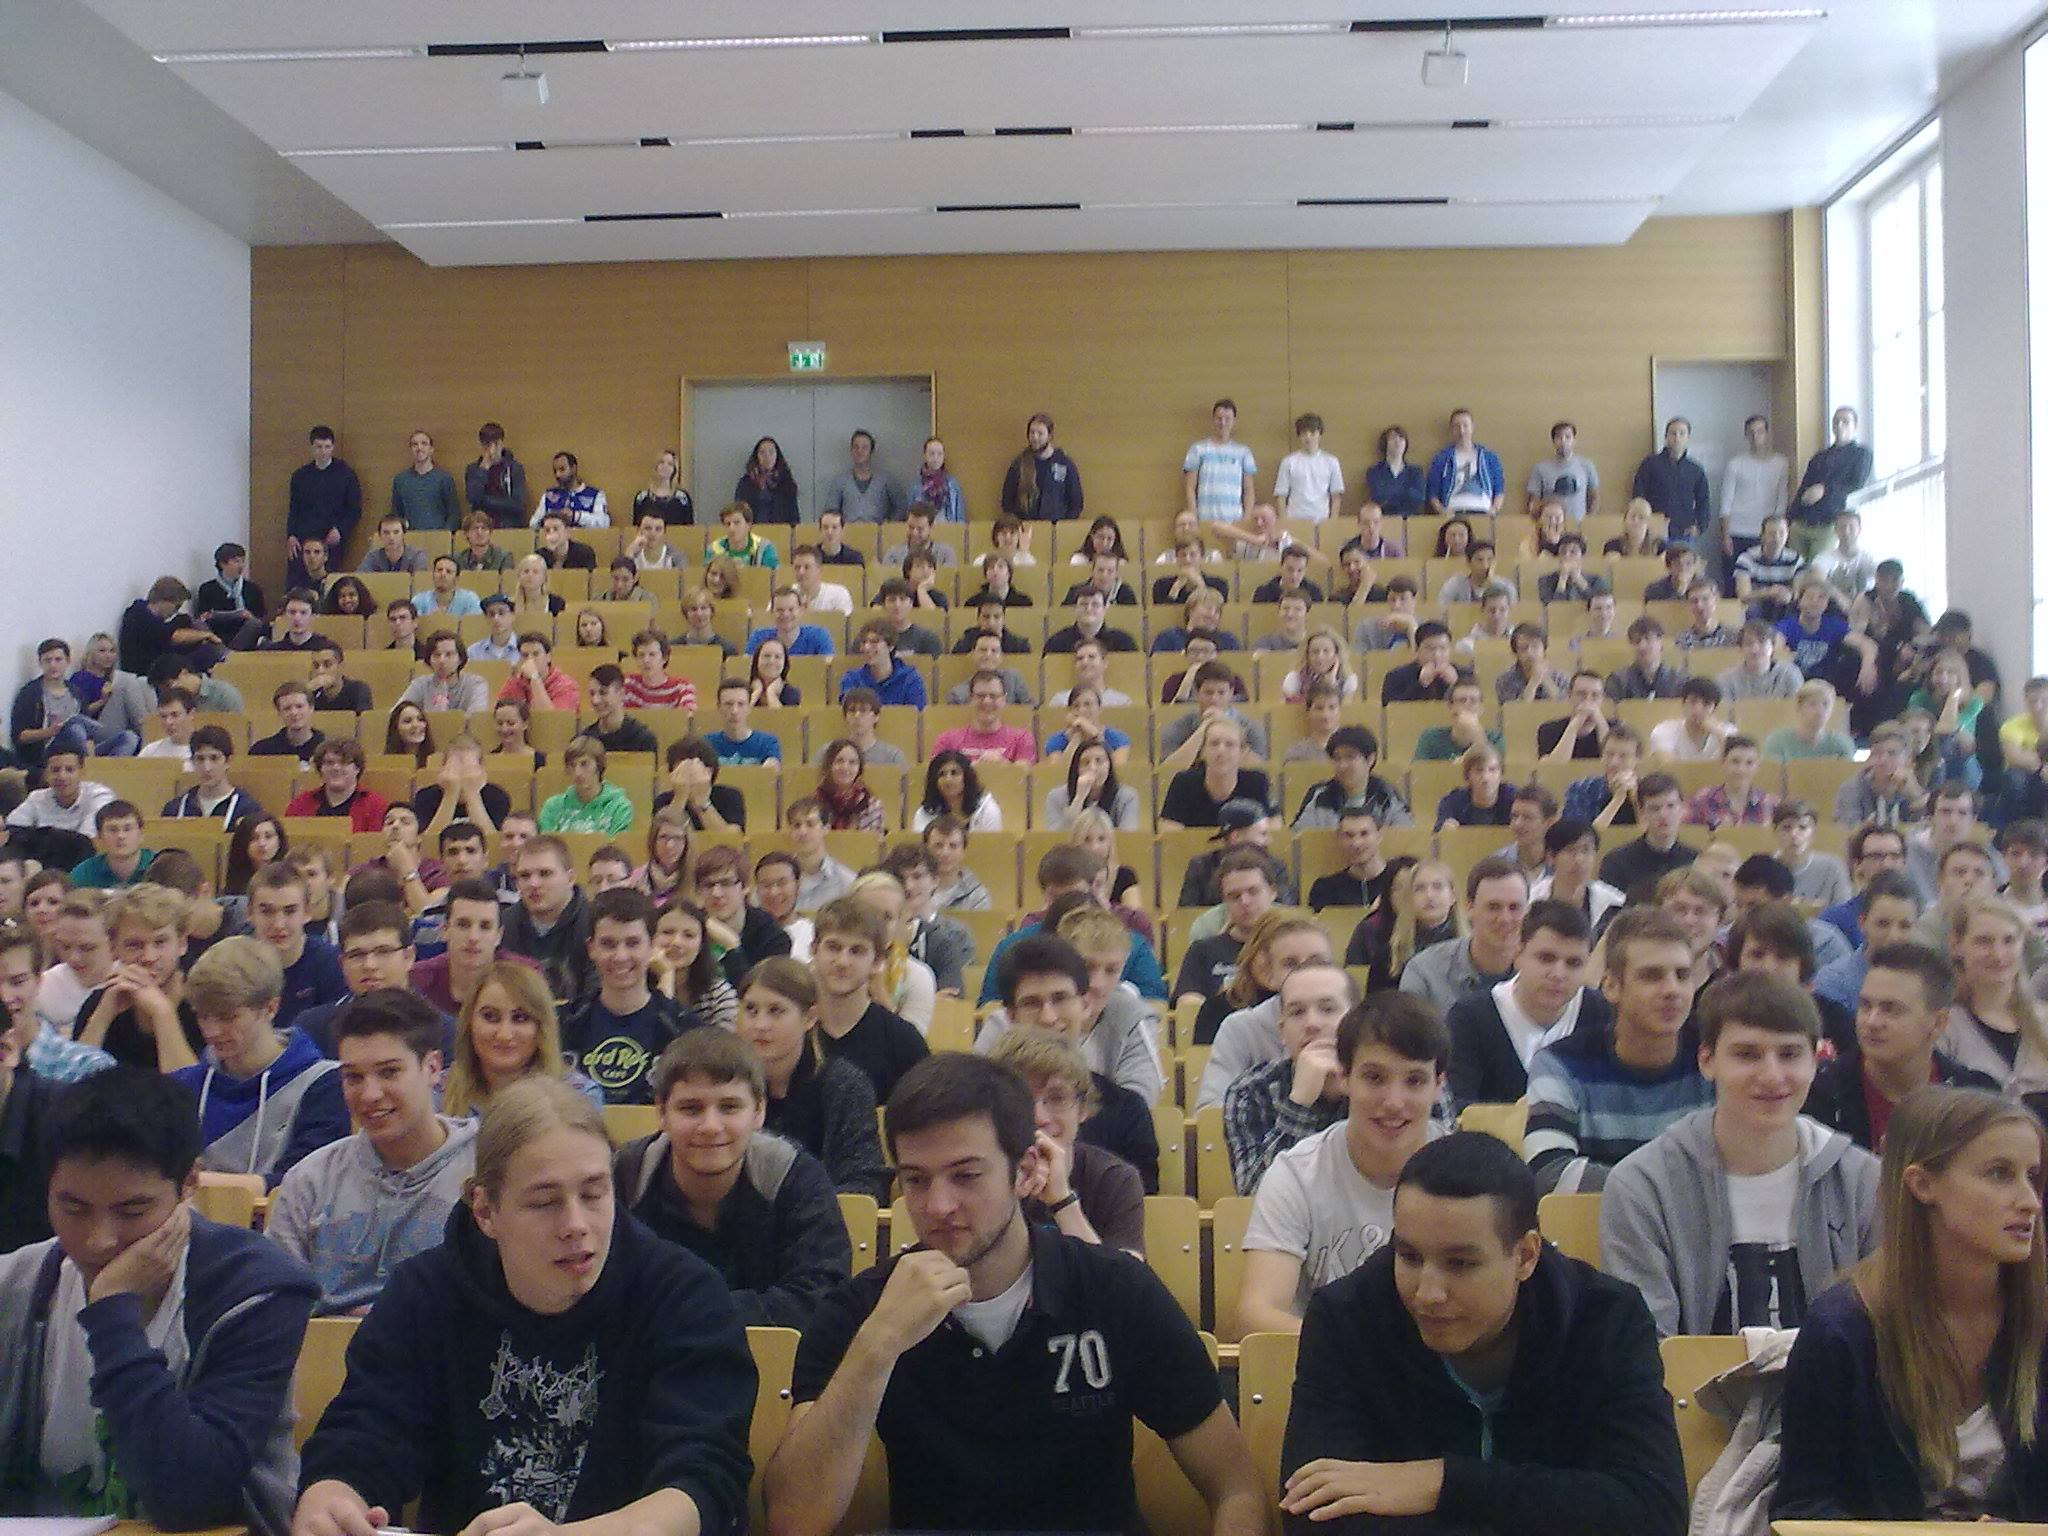
\includegraphics[scale=0.065]{ws14_15}
				\caption{WS 2013/2014}
			\end{figure}
		\end{column}
		\begin{column}{6cm}
			\begin{figure}
				\centering
				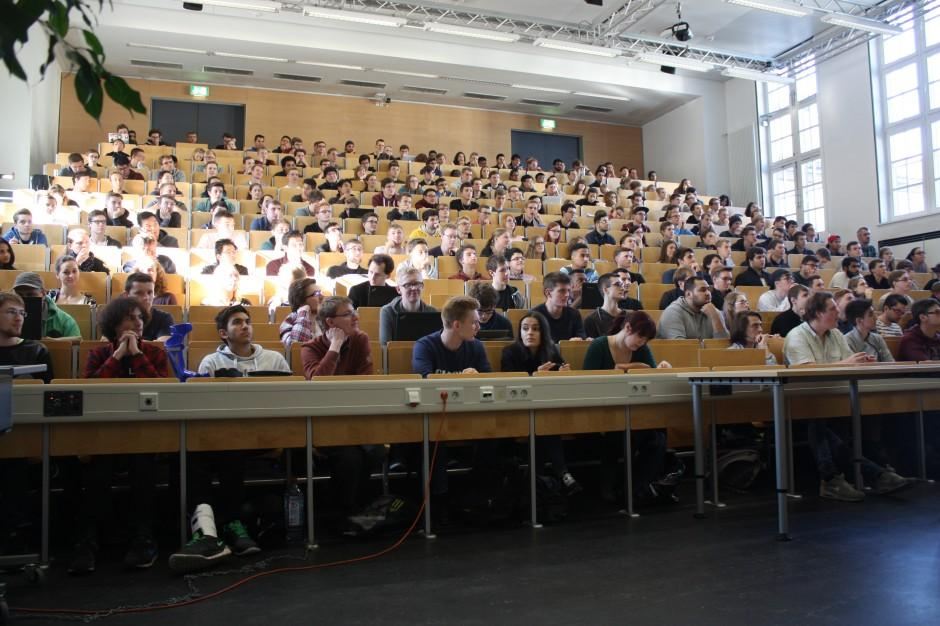
\includegraphics[scale=0.21]{ws16_17}
				\caption{WS 2016/2017}
			\end{figure}
		\end{column}
	\end{columns}

\end{titleframe}



\section{Veranstalter}
\subsection*{Fachschaft Informatik}
\begin{frame}
	\frametitle{\insertsectionhead \\ {\small \insertsubsectionhead}}
	\begin{itemize}
		\item "Die Schüler*innenvertretung der Studierenden"
		\item Bei Problemen zwischen Dozierenden und Studenten vermitteln
		\item Ansprechpartner für Studierende bei Fragen zum Studium
		\item Den Studienablauf am Fachbereich weiter verbessern
		\item Soziale Interaktion zwischen Studierenden fördern
		\item Erstsemestern den Einstieg ins Studium erleichtern
		\item ...
	\end{itemize}
\centering
\vspace{3mm}
\huge Mehr auf D120.de
\end{frame}

\section{Kontakt}
\begin{frame}
	\frametitle{\insertsectionhead \\ \insertsubsectionhead}
	\begin{itemize}
		\item \textbf{Mail:} \href{mailto:vorkurs@d120.de}{vorkurs@d120.de}
		\item \textbf{Moodle:}  \href{https://moodle.informatik.tu-darmstadt.de/course/view.php?id=624} {https://moodle.informatik.tu-darmstadt.de}
	\end{itemize}
	\vspace{3.5cm}
	\begin{alertblock}{Hinweise}
		Ihr habt allgemeine Fragen: Schreibt ins Moodle-Forum. \\
		Ihr habt spezielle Fragen an uns: Schreibt uns eine Mail.
	\end{alertblock}
\end{frame}

\section{Ablauf des Vorkurses}
\subsection{Ein üblicher Tag im Vorkurs}
\begin{frame}
	\frametitle{\insertsectionhead \\ {\small \insertsubsectionhead }}
	\begin{itemize}
		\item \textbf{Vormittags Vorlesung}
		\begin{itemize}
			\item interaktiv
			\item heißt: Fragen stellen
		\end{itemize}
		\item \textbf{Mittagspause}
		\begin{itemize}
			\item Mensa
			\item Leute kennenlernen
		\end{itemize}
		\item \textbf{Nachmittags Übung}
		\begin{itemize}
			\item Gruppenarbeit
			\item ergänzend zur Vorlesung
			\item in den Poolräumen der Uni
			\item offenes Ende
		\end{itemize}
		\begin{block}{Hinweis:}
			Heute ist keine Übung!
		\end{block}
	\end{itemize}
\end{frame}

\subsection{Wochenplan}
\begin{frame}
	\frametitle{\insertsectionhead \\ {\small \insertsubsectionhead}}
	\textbf{Allgemeines Programm}
	\begin{itemize}
		\item Montag (also Heute)
		\begin{itemize}
			\item Beginn um 14:15 Uhr
			\item S2|02 C205 (Hier)
		\end{itemize} 
		\item Dienstag, Mittwoch 
		\begin{itemize}
			\item Beginn um 10:15 Uhr
			\item S2|02 C205
		\end{itemize} 
		\item Freitag 
		\begin{itemize}
			\item Beginn um 11:45 Vorlesung
			\item S2|02 C205
		\end{itemize}
		\item Übertragung in S2|02 C110 und C120
		\item Übungen immer nach der Mittagspause - im C-Pool S2|02 C003 und im Lernzentrum S2|02 A020 (im Keller)
	\end{itemize}
\end{frame}

\subsection{Lageplan}
\begin{frame}
	\frametitle{\insertsectionhead \\ {\small \insertsubsectionhead}}

	\begin{columns}[T]
		\begin{column}{.4\textwidth}
			\begin{itemize}
				\setlength\itemsep{4em}
				\item \textbf{Robert-Piloty-Gebäude (Informatik)}
				\begin{itemize}
					\item S202 C205
					\item Poolraum
				\end{itemize}
				%Altes Hauptgebäude wird dieses Semester nicht verwendet.
				%aufgrund dessen wurde das item mit phantom und [] vor dem \item auf unsichtbar gestellt.
				\item[]\phantom{\textbf{Altes Hauptgebäude (Übertragung)}}

				\item \textbf{Mensa}
			\end{itemize}
		\end{column}

		\begin{column}{.6\textwidth}
			\vspace{-0.3cm}
			\hspace{1.0cm}
			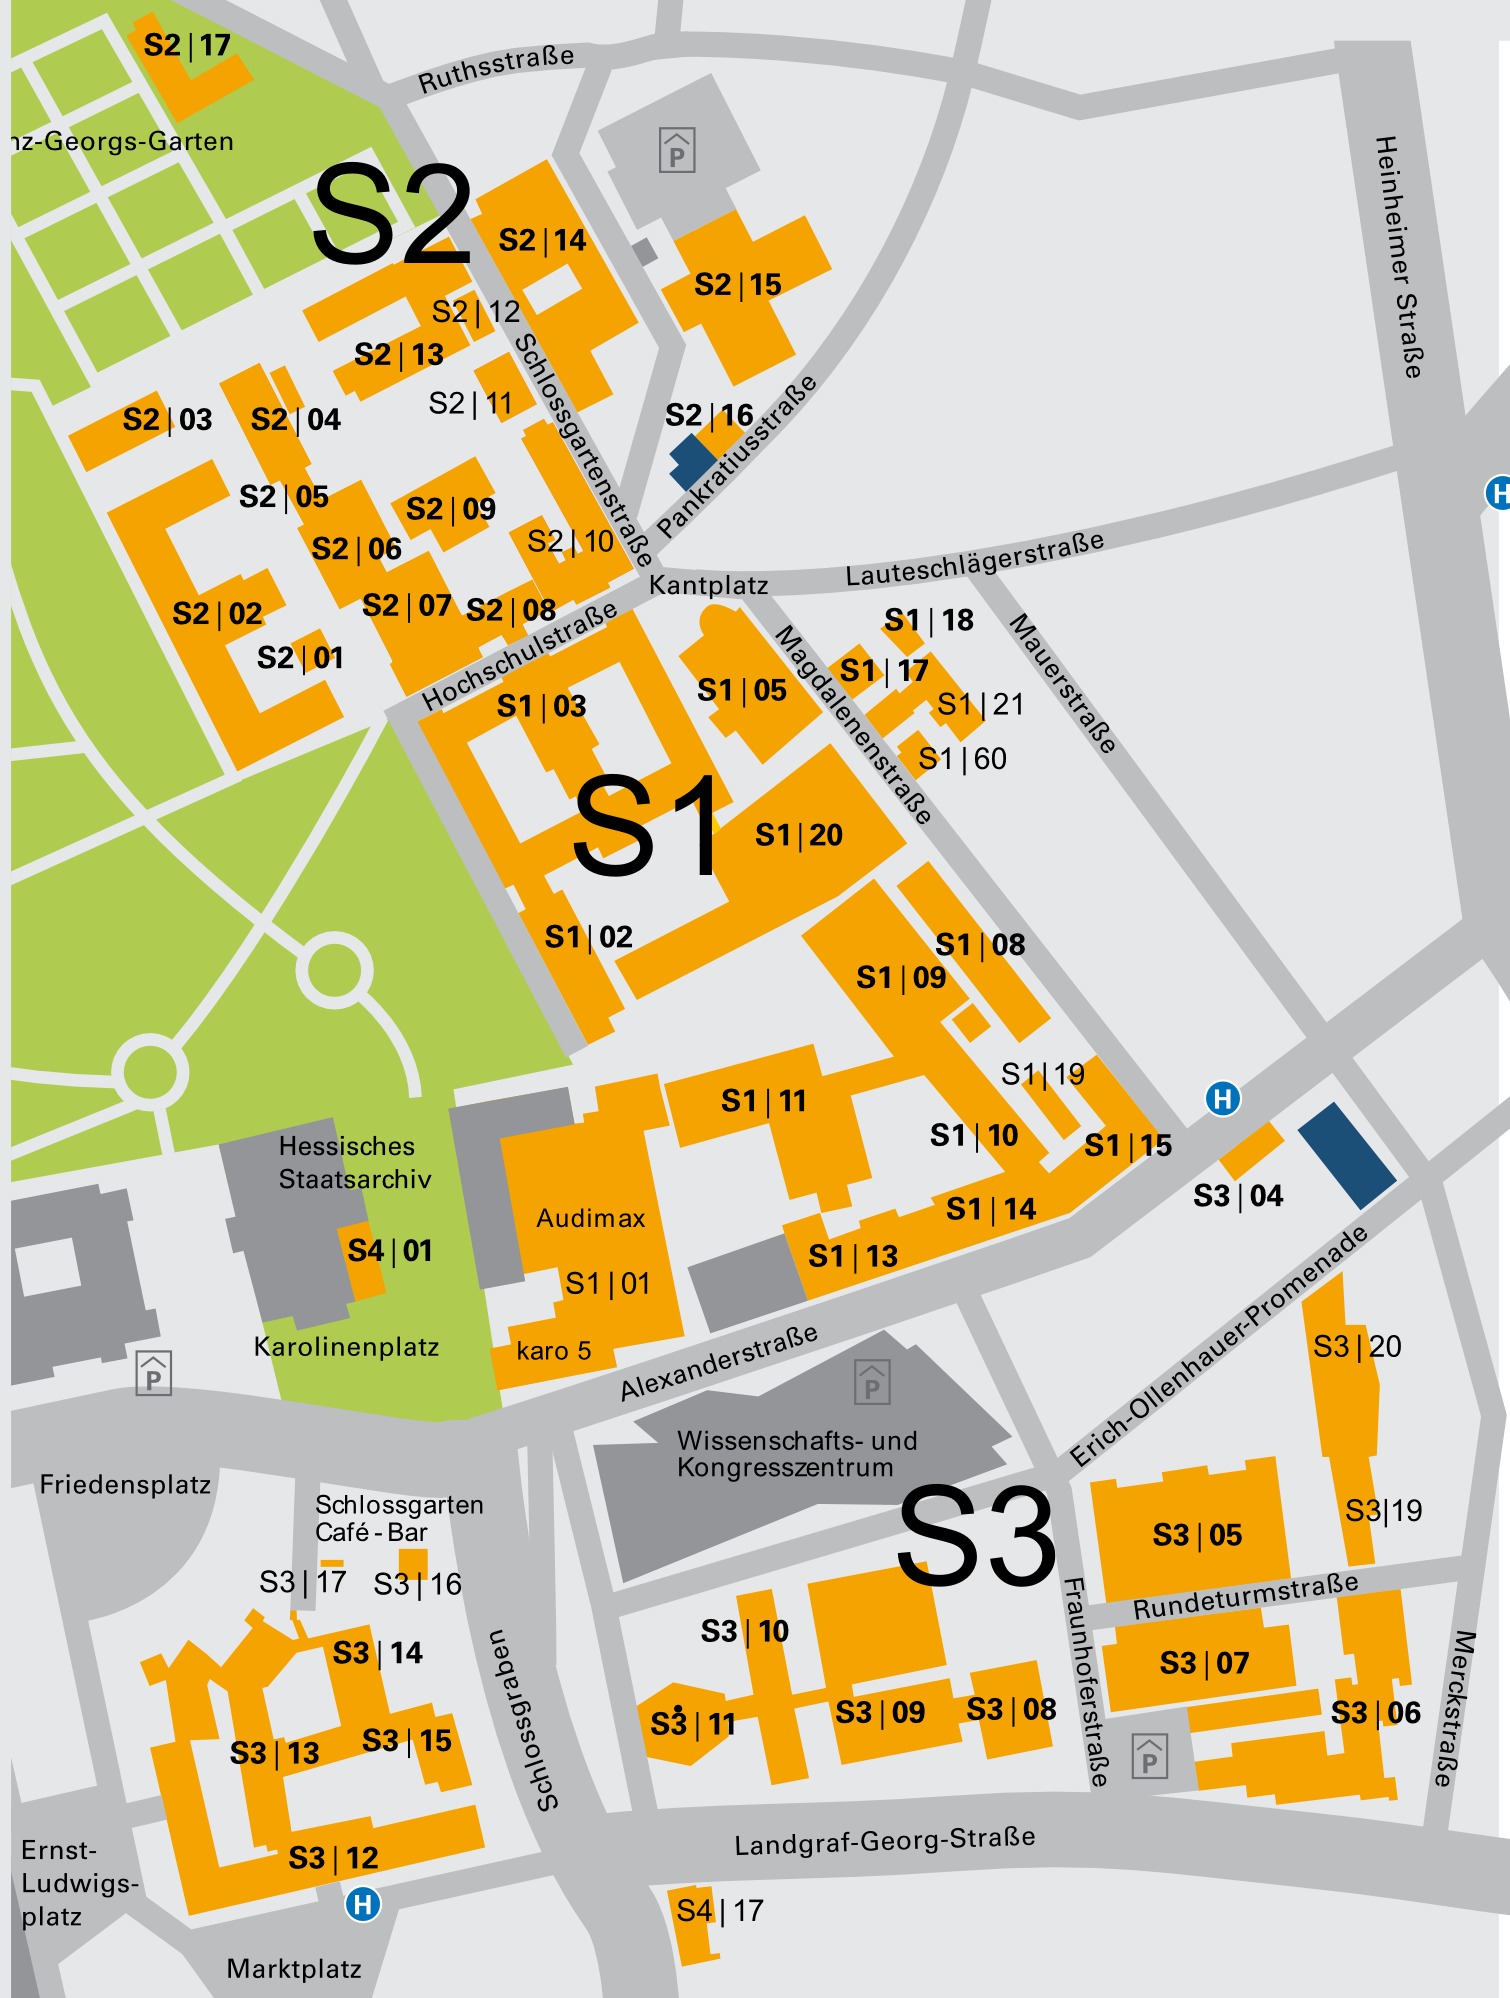
\includegraphics[trim={0.2cm 4.8cm 3cm 0.3cm}, clip,width=0.75\textwidth]{lageplan_blanko}
			\begin{tikzpicture}[overlay]
				%pfeile:
				%\draw[->,line width=3pt, tud3c](-7.2, 2.2)--(-2.5, 2.2); % altes Hauptgebäude
				\draw[->,line width=3pt, tud3c](-7.2, 5.2)--(-4.4, 2.9); % Piloty
				\draw[->,line width=3pt, tud3c](-9.7, 0.4)--(-1.2, 1.2); % Mensa
			\end{tikzpicture}
		\end{column}
	\end{columns}
\end{frame}

\subsection{Mensa}
\begin{frame}
	\frametitle{\insertsectionhead \\ {\small \insertsubsectionhead}}
	\begin{columns}
		\begin{column}{5cm}
			\begin{itemize}
				\item \textbf{Otto B.}
				\begin{itemize}
					\item Mo-Fr 11:15 - 14:00 Uhr
				\end{itemize}
				\item \textbf{Marktrestaurant}
				\begin{itemize}
					\item Mo-Do 11:00 - 14:30 Uhr
					\item Fr 11:00 - 14:00 Uhr
				\end{itemize}
				\item \textbf{Bistro Stadtmitte }
				\begin{itemize}
					\item Mo-Do 8:00 - 16:00 Uhr
					\item Fr 8:00 - 15:00 Uhr
				\end{itemize}
			\end{itemize}
			\begin{block}{Hinweis:}
				Bargeldaufschlag 0,20€! Keine Athenekarte? Ihr könnt eine Karte im Bistro leihen (5€ Pfand).
			\end{block}
		\end{column}
		\begin{column}{7.2cm}
			\vspace{-2.5ex}
			\begin{figure}
				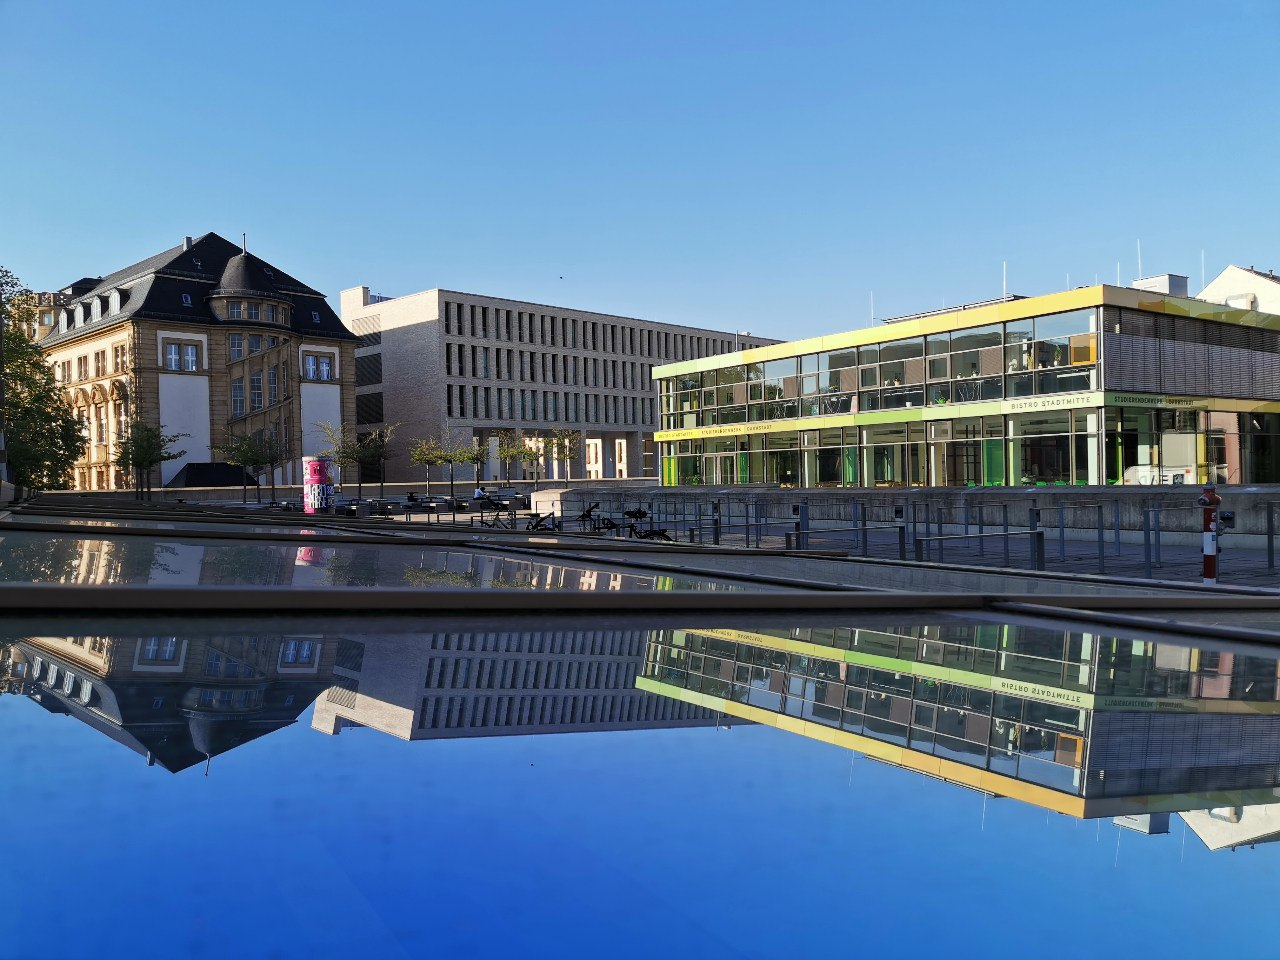
\includegraphics[width=0.75\textwidth]{mensa2}
				\caption{Mensa Stadtmitte (das bunte Gebäude)}
			\end{figure}
		\end{column}
	\end{columns}
\end{frame}


\subsection{Stoffplan}
\begin{frame}
	\frametitle{\insertsectionhead \\ {\small \insertsubsectionhead}}
	\begin{itemize}
		\item Wie fängt man Programmieren an?
		\item Was ist Python?
		\item Mein erstes Programm
		\item Datentypen und Operatoren
		\item Schleifen und bedingte Anweisungen
		\item Funktionen \& Rekursion
	\end{itemize}
\end{frame}

\subsection{Voraussetzungen}
\begin{frame}
	\frametitle{\insertsectionhead \\ {\small \insertsubsectionhead}}
	\centering
	\vspace{2.5cm}
	\Huge Keine 
\end{frame}

\subsection{Ziele}
\begin{frame}
	\frametitle{\insertsectionhead \\ {\small \insertsubsectionhead}}
	\begin{itemize}
		\item Vereinfachter Start ins Studium
		\item Grundlegende Konzepte verstehen
		\item Leute Kennenlernen
		
	\end{itemize}
\end{frame}

\subsection{Übungsaufgaben}
\begin{frame}
	\frametitle{\insertsectionhead \\ {\small \insertsubsectionhead}}
	\begin{itemize}
		\item Aufgaben mit unterschiedlichen Schwierigkeitsgrad
		\item Tutor*innen im Poolraum, die euch unterstützen
		\item Helft euch gegenseitig, denn so lernt ihr am meisten
		\item Ihr müsst nicht alle Aufgaben lösen
	\end{itemize}
\end{frame}

\subsection{Material}
\begin{frame}
	\frametitle{\insertsectionhead \\ {\small \insertsubsectionhead}}
	\begin{itemize}
		\item Vorlesungsfolien \& Übungen
		\item Ankündigungen
		\item Fragen, Foren
	\end{itemize}

	\begin{block}{Lernportal Informatik - Vorkurs}
		\vskip 10 pt
		\Huge{Gastschlüssel:} \textbf{9102srukroV}\\
		\normalsize
		\vskip 8 pt
		Nähere Informationen zum Zugriff auf die Materialien:\\
		\quad \href{https://d120.de/vorkurs}{https://d120.de/vorkurs}
	\end{block}
\end{frame}

\section{Ophase}
\begin{frame}
	\frametitle{\insertsectionhead \\ {\small \insertsubsectionhead}}
	\textbf{Nächste Woche} ist die Ophase (7. bis 11.10.2018)! \\
	Nehmt auf jeden Fall daran teil. Es lohnt sich für euch!
	\begin{figure}
		\centering
		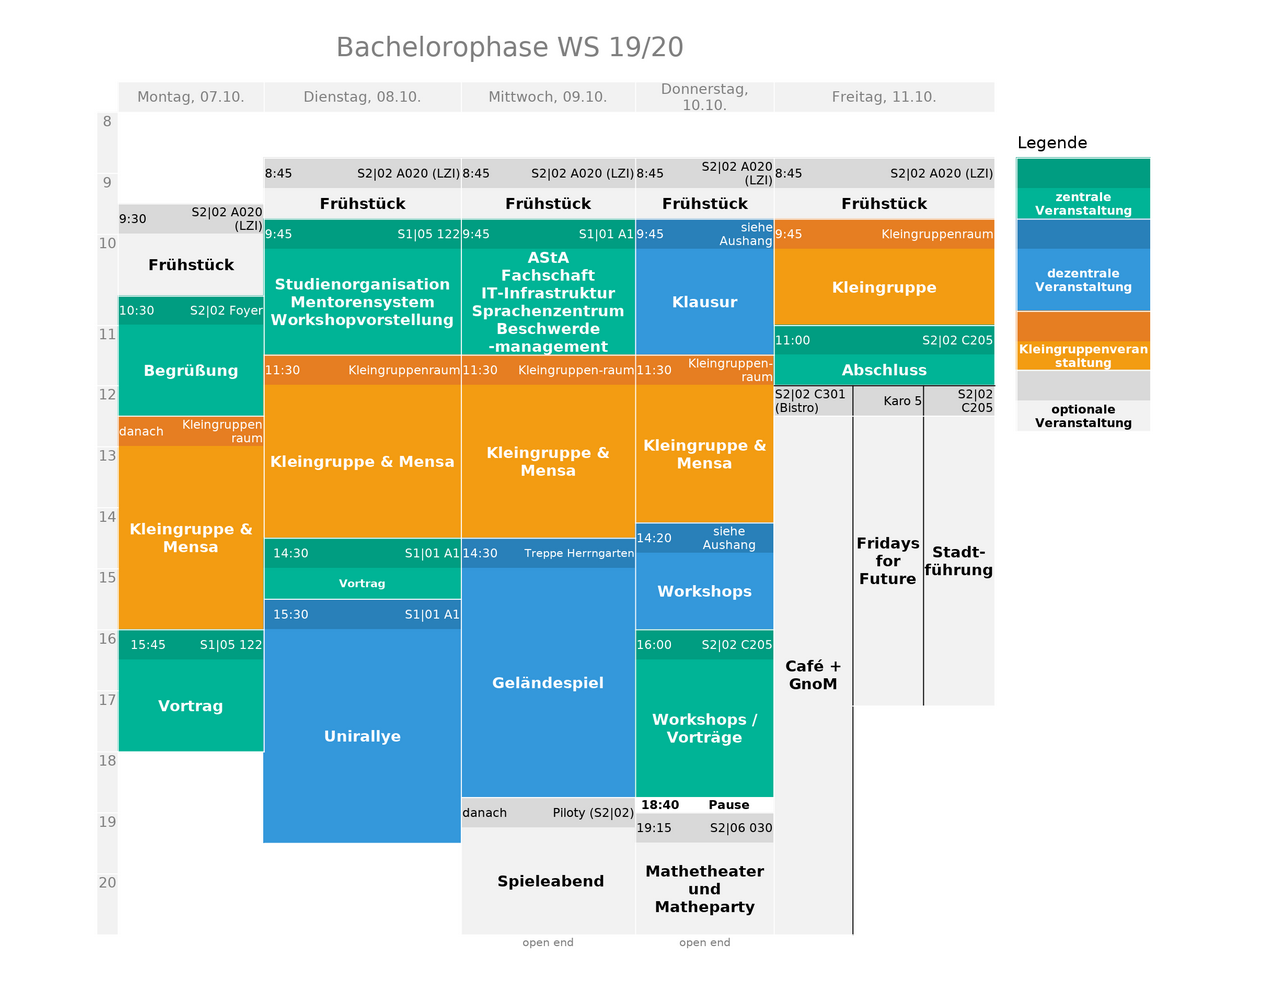
\includegraphics[scale = 0.14]{ophase}
	\end{figure}
\end{frame}

\end{document}
